\documentclass[a4paper, onecolumn, 12pt]{article}
\usepackage[left=33mm,right=33mm,top=35mm,columnsep=15pt]{geometry} 

% basic packages
\usepackage[english]{babel} %language
\usepackage[utf8]{inputenc} %input encoding
\usepackage{float} %position of floating objects
\usepackage{bookmark} %hyperlinks in pdf
\usepackage{subcaption}
\usepackage[T1]{fontenc}
\usepackage{lipsum} %placeholder text

% math packages
\usepackage{amsthm} %theorems
\usepackage{amsmath} %math
\usepackage{mathtools} %still math

% code packages
\usepackage{listings} %code
\usepackage{xcolor} %syntax highlighting
\usepackage{algorithm}
\usepackage{algpseudocode}
\usepackage{fancyvrb}

% todonotes package
\usepackage{xkeyval}
\usepackage{tikz}
\usepackage{calc}
\setlength {\marginparwidth }{2cm}
\usepackage{todonotes} % Load the todonotes package

% custom commands
\newcommand\tab[1][.3cm]{\hspace*{#1}}
\newcommand\tabeq[1][.5cm]{\hspace*{#1}}

% \usepackage{physics}
% \usepackage{adjustbox}
% \usepackage{placeins}
% \usepackage{csquotes}
% \usepackage[normalem]{ulem}
% \useunder{\uline}{\ul}{}

\title{Remote Interaction with a Nao Humanoid in competitive games \\ Elective in AI / HRI Report}
\author{Flavio Maiorana \and Valerio Spagnoli \and Flavio Volpi}
\date{\today}

\begin{document}

\maketitle

\section{Introduction}
\label{sec:intro}

In the context of RoboCup games, robots are fully autonomous. However, they
surely could benefit from interaction with humans. For example, human soccer
players benefit from receiving suggestions and sometimes even explicit
instructions on what to do during the match. Similarly, an autonomous soccer
robot could receive informed suggestions to enhance its planning
\todo[inline]{Andrebbe detta meglio sta cosa}. In this project, we aim to make a
small step in that direction by developing a system that allows a human operator
to remotely control and interact with a Nao Humanoid through a graphical
interface. 

\subsection{Context and Motivation}
\label{sec:context}

Receiving instructions from a coach can be a game-changer in a soccer match. And
also, receiving feedback from the robot when issuing a command drastically
improves the interaction quality. This project was specifically designed to be
used in the RoboCup 2024 SPL challenge, where two robots of one team had to
compete against two robots of the opponent team, and one of the two robots for
each team was controlled by a human operator. Furthermore, the rules of the
challenge forced the human operator to turn his back to the field, in order to
not directly observe the environment. This constrained us to make use of the
directional robot-human communication also for the reconstruction of the world
model.

\todo[inline]{Qua si puó dire di piú}


\subsection{Objectives}
\label{sec:obj}

The main objective of the project is to develop a framework that allows the human operator
to use the robot as a proxy to interact with the environment, namely the soccer
field. To do this, a form of bidirectional interaction between the human operator 
and the controlled robot is necessary. The human needs
to be completely aware of the robot's surroundings, that is, the human can
perceive the robot's surroundings only through the robot's sensors. The robot,
on the other hand, has to be able to receive commands from the human operator
and execute them in real-time. The robot should also be able to send feedback to
the human operator in real-time. 
\todo[inline]{Allungare un po' il brodo}
\todo[inline]{Spingerei anche sul fatto che il tutto deve essere utilizzabile in un 
ambiente competitivo}

\subsection{Summary of the results}
\label{sec:summary}

Our system achieved the objective of allowing a human operator to control a Nao
by voice and using a graphical interface, and to receive feedback from the robot
in response to the commands. The system integrates various modules, such as:
\begin{itemize}
    \item \textbf{Communication}, which manages the communication between the robot and
    the human operator
    \item \textbf{Mental model}, responsible for representing the field by
    accessing only the robot's perceptions
    \item \textbf{Interaction}, by answering to the commands before executing
    them, considering also the feasibility of the execution itself
    \item \textbf{Memory}, the past command is held in memory, in order to
    resume it in case it is needed
\end{itemize}
The system was tested in the RoboCup 2024 SPL challenge, where SQPR Team reached
the third place, demonstrating the effectiveness of the system in a competitive
environment.

\newpage

\section{Related Work}
\label{sec:rel}

Interpreting human signals has been a challenge for some time now in Robotics.
Humans communicate through various modalities, including vision, audio, and
motion. This multimodal nature provides rich information that sensory inputs can
capture and analyze. 

Recent advances in Deep Learning have facilitated the
integration of multimodal data, significantly improving the comprehension of
relationships within individual modalities, a key factor for precise message
interpretation \cite{LIU20183} \cite{su2023recent}.

In RoboCup Soccer, human-robot interaction is predominantly one-way, with human
referees conveying game states and events to robots. A significant trend in the
RoboCup SPL is the progressive reduction of network communication in
favor of human-like signal interpretation, allowing robots to interpret human
signals more naturally. \cite{digiambattista}

A notable case worth to mention is also \cite{antonioni}, where they propose an
approach to improve the decision making process through the audience noise by
extracting relevant features through MFCC coefficients and applying a
reinforcement learning pipeline. 

This case could fall into a broader category where the goal is to improve the
communication from an ideal coach to the robot in order to improve planning and
decision-making. In particular, \cite{musumeci} tackles this problem by
designing a system that enriches the planning process with temporal goals and
constraints given by human indications. 

Our work is inspired by these studies, and the goal is to develop a system that
allows a human operator to have a one-to-one interaction with a robot, acting
like a coach in a soccer match.

\newpage
\section{Solution}
\label{sec:sol}

The system can be divided in two main parts: the framework backbone, written in
C++, which runs on the robot itself, and the interface, written in Python and
Nodejs, responsible for issuing commands to the robot and receiving feedback or
sensory information. 

\subsection{Framework backbone}
The framework on which everything stands on is derived from that one of the
German team B-Human \cite{bhuman2023}, University of Bremen. At low level, the robot is 
controlled by three threads:
\begin{itemize}
    \item Cognition: it is responsible for collecting all informations from the 
    environment through cameras and sensors; also, it takes images and informations as input,
    and returns high level commands about the actions the robot has to execute;
    \item Motion: it converts high level commands of the thread Cognition in effective
    motion of the robot;
    \item Debug: it allows a communication between the robot and the host pc for the 
    transmission of debugging information.
\end{itemize}
\todo[inline]{aggiungere immagine dei processi}

The two main components for the collection and storage of information from the environment
are called Representations and Modules.
Representations store informations at the current instant, and they represent the actual overview
of the world. Each representation is a derived class of the class $Streamable$, which allows a 
direct connection of all attributes and functions of the given representation with all other
representations and modules. Furthermore, each representation has a single module provider, which
is the only capable of modifying its attributes.

Instead, the task of the modules is to make computations which require specific inputs and returns
determined output. In details, a module can specify the representations it needs in input through
the macros REQUIRES and USES, and must specify the representations it is going to modify through
the macro PROVIDES. A module must specify a function named $update$, that has the scope to 
perform the real updates of the informations inside the provided representations

The correct usage of REQUIRES and USES is established by a scheduler inside the software, which decides 
which is the right execution order of the modules according to cyclic dependencies between representations.
For example,
\todo[inline]{@FLAVIO V. : inserire esempio di moduli/rappresentazioni}

\begin{figure}
    \centering
    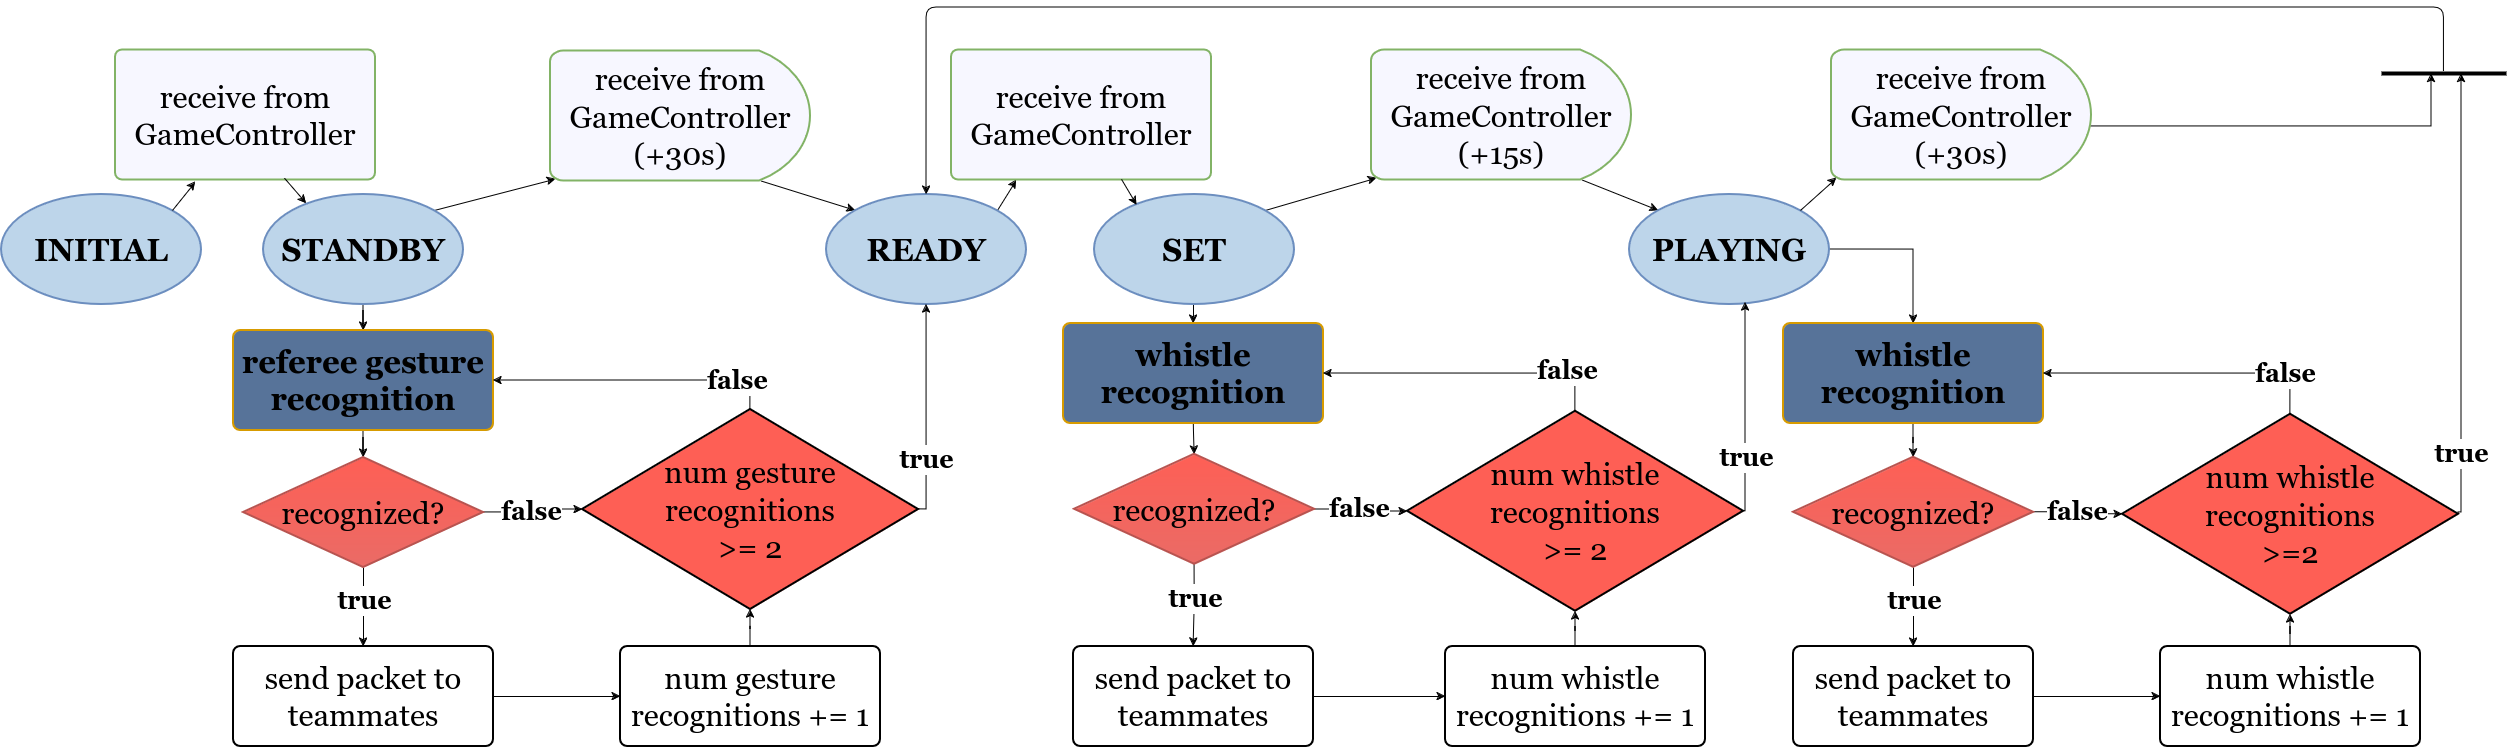
\includegraphics[width=0.9\linewidth]{assets/flowchart.png}
    \label{fig:flowchart}
    \caption{Complete pipeline of the game states}
\end{figure}

\subsubsection{Memory}

\todo[inline]{Boh}

\subsubsection{Social Reasoning}

An important aspect of RoboCup SPL games are the game rules. These are conceived
from year to year to shift the games to be more realistic. If we want, they
could be considered as a form of social rules which the robots need to obey to
while playing. Depending on the game state, some actions are not permitted. For
instance, in SET the robots are not allowed to move. Similarly, one could impose
a rule that avoids the robot to score in its own goal, even if it is requested
to. Of course, in order to to some adequate social reasoning, it is necessary
for the robot to have a sufficiently detailed model of the game state and the
field.

\subsubsection{Mental Modeling}

\todo[inline]{Come rappresenta il mondo il robot? Stato del gioco e del campo fisico}



\subsection{Interface}

We opted for a solution that prioritizes high-level commands and audio-visual
feedback. The graphical interface is made by a bunch of buttons, that allow the
human operator to send commands to the robot, and a 2D representation of the
field that shows the robot's position and its recosntruction of the world.  

\begin{figure}[H]
    \centering
    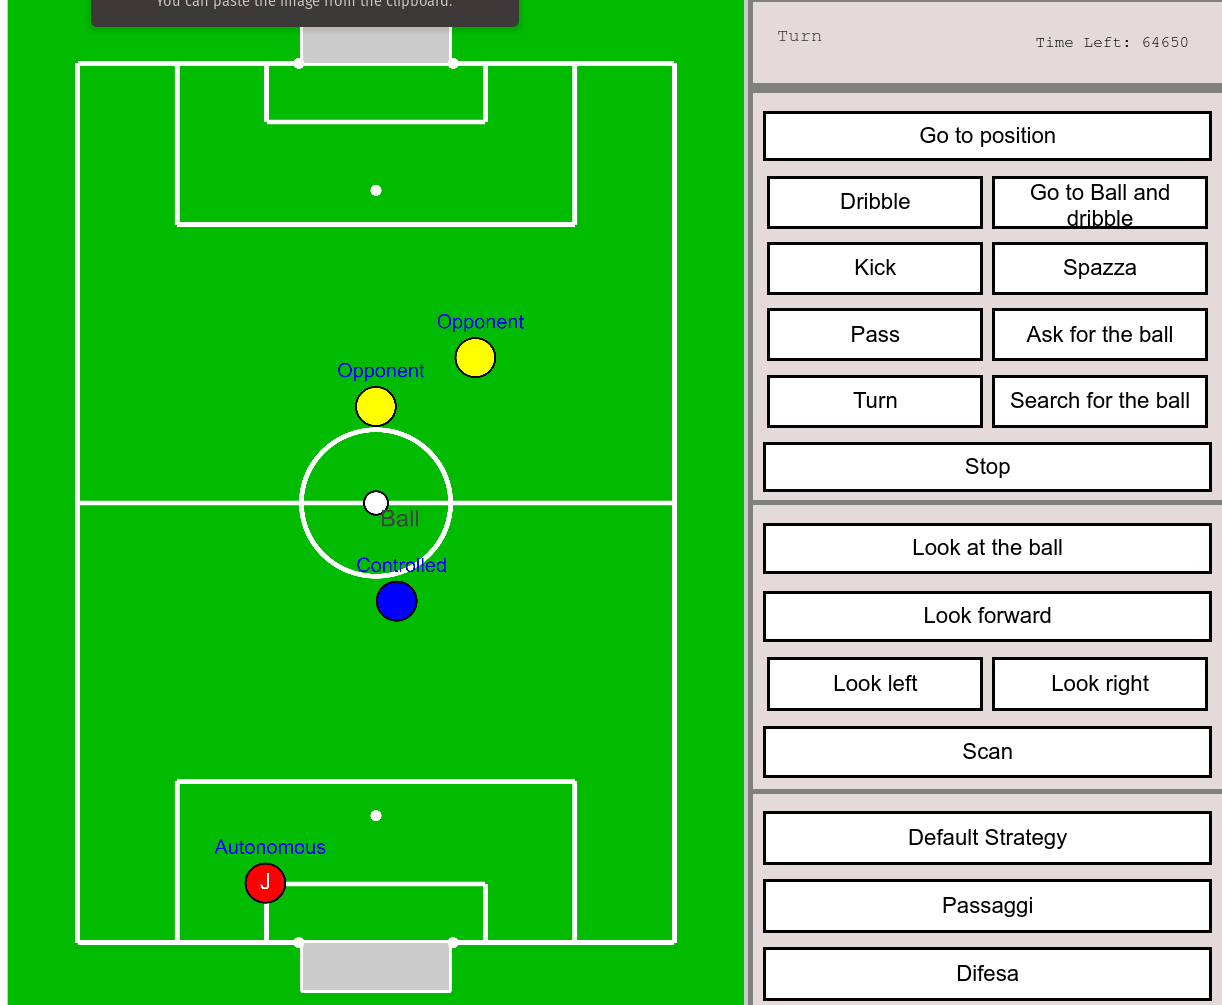
\includegraphics[width=0.9\linewidth]{assets/interface.png}
    \caption{The graphical interface}
    \label{fig:interface}
\end{figure}

\begin{figure}[H]
    \centering
    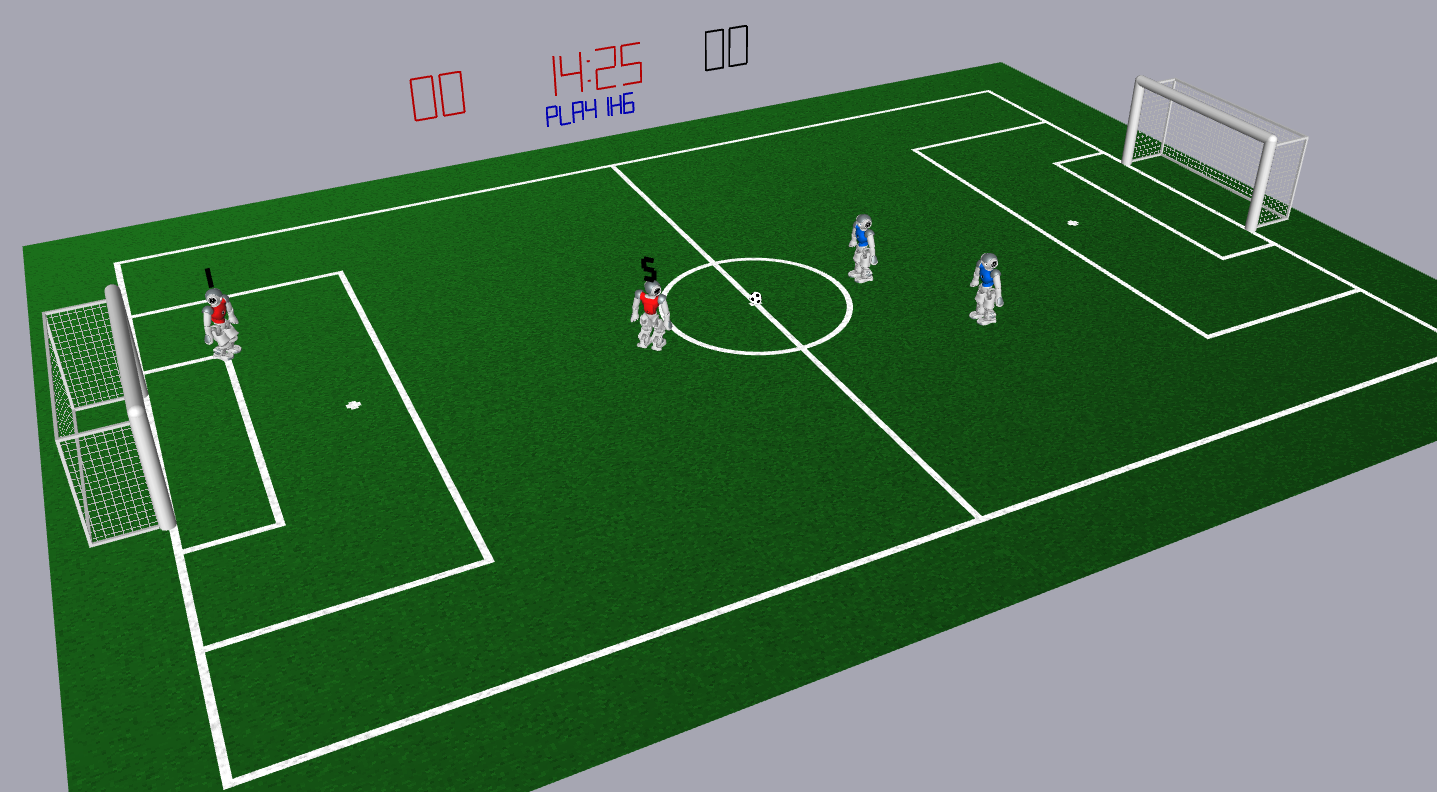
\includegraphics[width=0.9\linewidth]{assets/simrobot.png}
    \caption{The Corresponding Field Configuration}
    \label{fig:nao}
\end{figure}

\newpage
\section{Implementation}
\label{sec:impl}

From an implementative point of view, the system can be divided in four modules: 
\begin{itemize}
    \item \textbf{Communication Layer}: exchanges messages between the robot and the human operator
    \item \textbf{Framework}: the backbone of the system, which runs on the robot
    \item \textbf{GUI}: the graphical interface that allows the human operator to interact with the robot
    \item \textbf{Speech-to-Text Module}: the module that converts the human operator's voice commands to text
\end{itemize}

These modules are wrapped around the two main data structs that encapsulate the
exchanged messages, namely the \textit{HumanCommand} struct and the
\textit{DebugInfo} struct. The former is used to send commands from the human
operator to the robot. It has the following structure:
\begin{verbatim}
    1B: Command body
    1B: Command head
    1B: Strategy
    8B: [pos_x, pos_y]
    command_format: "<BBBff"
\end{verbatim}

Basically, it is formatted as a tuple of 5 elements, where the first three are
Bytes and the last two are floats. The last two elements are the coordinates of
the target position, which are indicated on the 2D field. This precise structure
is needed to be able to send the command through the socket and parse it on the
C++ side.

The \textit{DebugInfo} struct, on the other hand, is used to send feedback from
the robot to the human operator. It has the following structure:

\begin{verbatim}
1)      4B header
2)      1B version
3)      1B player_num
4)      1B team_num
5)      1B fallen
6-9)    3f (12B) [pos_x, pos_y, theta]
9)      1f (4B) ball_age
10-12)  2f (8B) [ball_pos_x, ball_pos_y]
12)     1H (2B) num_of_data_bytes
13)     1B player_role
14)     1B current_obs_size
15-35)  20B obstacle_types  
35-55)  20f (80B) obs_center_x
55-75)  20f (80B) obs_center_y
75-95)  20f (80B) obs_last_seen
95)     1H (2B) message_budget
96)     1H (2B) secs_remaining
97-99)  2B arm_contact
99-101) 2B arm_push_direction
101-103)2f (8B) arm_time_of_last_contact
103)    2f (8B) padding (whistle)
104-106) 2f (8B) teamball
106-108) 2f (8B) teamballvel
108)    12B padding

data_format: "<d4sBBBB3ff2fHBB20B20f20f20fHH2B2B2f2f2f2f12B"
\end{verbatim}

This data packet contains all the information that is needed to have a graphical
representation of the robot's mental model of the field. \todo[inline]{Spiegare un po'}

\subsection{Communication Layer}

The communication layer is responsible for the exchange of messages between the
robot and the human operator. It is written in Python and based on UDP sockets. 

\begin{verbatim}
def send_command_to_cpp(self, command: int, strategy: int, x: int, y: int):
    if command_number > self.config.command_offset:
        command_body_number = Command.Null.value
        command_head_number = command_number - self.config.command_offset
    else:
        command_body_number = command_number
        command_head_number = Command.Null.value
    encoded_data = struct.pack(
        self.config.command_format,
        command_body_number,
        command_head_number,
        strategy_number,
        x_position,
        y_position
    )
    try:
        client_socket.sendto(encoded_data, (robot_ip, command_send_port))
        print(f"Sending message to C++: {encoded_data}")
    except Exception as e:
        print(f"Error in send_message: {e}")
\end{verbatim}

This function sends a command that is received from the GUI to the robot. The
receive function from nodejs is the following:

\begin{verbatim}
def receive_command_from_js(self) -> tuple[int, int, int, int]:
    try:
        data, addr = self.server_socket.recvfrom(1024)
    except Exception as e:
        print(f"Error in receiving the message: {e}")
    try:
        message = data.decode()
    except UnicodeDecodeError:
        print(f"Received non-UTF-8 message from JavaScript: {data} from {addr}")
    message_split = message.split('|')[1]
    content_message = message_split.split(',')
    task_type = content_message[2]
    command_number = Command[task_type].value
    strategy_number = int(content_message[5])
    task_label = content_message[4]
    selection = content_message[1]
    print(f"Task Label: {task_label}")
    if selection == "selection":
        x_position = int(content_message[6])
        y_position = int(content_message[7])
        print(f"X Position: {x_position}")
        print(f"Y Position: {y_position}")
    else:
        x_position = 0
        y_position = 0
    return command_number, strategy_number, x_position, y_position
\end{verbatim}
Basically, the python scripts receives a command in form of a string from the
GUI, unpacks it, puts it into a serialized format and sends it to the robot.


\subsection{Framework}

The framework is the backbone of the system. The two main functions are the
update of the CommandReceiver and the update of the DebugMessageHandler (which
sends sensory information). The CommandReceiver is responsible for updating the
representation HumanCommand, while giving some audio feedback to the human about
the received command. In the following function, the command is parsed,
converted to enums and stored in the HumanCommand representation. 

\begin{verbatim}
void CommandReceiver::update(HumanCommand& command) {
  
  if (theRobotInfo.number != RobotInfo::RoleNumber::controlled) return;
  
  char buffer[BUFFER_SIZE];
  int n = socket_read.read(buffer, BUFFER_SIZE);
  
  // First field (command_body): unsigned char
  HumanCommand::CommandBody received_command_body = 
      static_cast<HumanCommand::CommandBody>(buffer[0]);
  
  // Second field (command_head): unsigned char
  HumanCommand::CommandHead received_command_head = 
      static_cast<HumanCommand::CommandHead>(buffer[1]);
  
  // Third field (strategy): unsigned char
  HumanCommand::Strategy strategy = 
      static_cast<HumanCommand::Strategy>(buffer[2]);
  
  // Fourth field (x_pos): int (4 bytes)
  float x_pos;
  std::memcpy(&x_pos, buffer + 3, sizeof(x_pos));
  
  // Fifth field (y_pos): int (4 bytes)
  float y_pos;
  std::memcpy(&y_pos, buffer + 7, sizeof(y_pos));
  
  if (n > 0) {
      SystemCall::say(HumanCommand::CommandBody2String(received_command_body));
  
      if(received_command_body != HumanCommand::CommandBody::BaseCommandBody){
          command.commandBody = received_command_body;
          command.x = x_pos;
          command.y = y_pos;
      }
      if(received_command_head != HumanCommand::CommandHead::BaseCommandHead)
          command.commandHead = received_command_head;
  
      command.strategy = strategy;
  }
  return;
}
\end{verbatim}

Once the command is stored in the HumanCommand representation, it is used by the
specific behavior we designed for the interacting robot. The update function
iterates over the possible commands (defined as an enumeration) in the start
state with a switch, executing the corresponding skill for each command. For
instance:

\begin{verbatim}
state(pass)
{
    transition
    {
    if (theHumanCommand.commandBody != HumanCommand::CommandBody::Pass)
        goto start;
    }

    action
    {
    int num = theTeamData.numberOfActiveTeammates;
    int size = theTeamData.teammates.size();
    if(num > 0){
        theSaySkill("Pass the ball");
        Vector2f target = theTeamData.teammates[0].theRobotPose.translation;
        KickInfo::KickType kickType = theLibPass.getKickType(target);
        float distance = theLibMisc.distance(target, theRobotPose);
        theGoToBallAndKickSkill(calcAngleToTarget(target), 
            kickType, true, distance);
    }
    else{
        theSaySkill("Go to ball and dribble");
        theGoToBallAndDribbleSkill(calcAngleToTarget(
            theLibStriker.strikerMovementPoint()));
    }
    }
}
\end{verbatim}

Whenever a new command is received, the robot answers with an audio feedback and
reiterates over the command list. 


\subsection{Speech-to-Text Module}

\todo[inline]{Blablabla}

\subsection{Interface}


\section{Results}
\label{sec:res}

\todo[inline]{Blocco 6 delle slide di iocchi}

\section{Experimental Evaluation} 

\section{Conclusion}
\label{sec:con}

\todo[inline]{Amen}

\bibliographystyle{unsrt}
\bibliography{references}

\end{document}
